
%% bare_conf.tex
%% V1.3
%% 2007/01/11
%% by Michael Shell
%% See:
%% http://www.michaelshell.org/
%% for current contact information.
%%
%% This is a skeleton file demonstrating the use of IEEEtran.cls
%% (requires IEEEtran.cls version 1.7 or later) with an IEEE conference paper.
%%
%% Support sites:
%% http://www.michaelshell.org/tex/ieeetran/
%% http://www.ctan.org/tex-archive/macros/latex/contrib/IEEEtran/
%% and
%% http://www.ieee.org/

%%*************************************************************************
%% Legal Notice:
%% This code is offered as-is without any warranty either expressed or
%% implied; without even the implied warranty of MERCHANTABILITY or
%% FITNESS FOR A PARTICULAR PURPOSE!
%% User assumes all risk.
%% In no event shall IEEE or any contributor to this code be liable for
%% any damages or losses, including, but not limited to, incidental,
%% consequential, or any other damages, resulting from the use or misuse
%% of any information contained here.
%%
%% All comments are the opinions of their respective authors and are not
%% necessarily endorsed by the IEEE.
%%
%% This work is distributed under the LaTeX Project Public License (LPPL)
%% ( http://www.latex-project.org/ ) version 1.3, and may be freely used,
%% distributed and modified. A copy of the LPPL, version 1.3, is included
%% in the base LaTeX documentation of all distributions of LaTeX released
%% 2003/12/01 or later.
%% Retain all contribution notices and credits.
%% ** Modified files should be clearly indicated as such, including  **
%% ** renaming them and changing author support contact information. **
%%
%% File list of work: IEEEtran.cls, IEEEtran_HOWTO.pdf, bare_adv.tex,
%%                    bare_conf.tex, bare_jrnl.tex, bare_jrnl_compsoc.tex
%%*************************************************************************

% *** Authors should verify (and, if needed, correct) their LaTeX system  ***
% *** with the testflow diagnostic prior to trusting their LaTeX platform ***
% *** with production work. IEEE's font choices can trigger bugs that do  ***
% *** not appear when using other class files.                            ***
% The testflow support page is at:
% http://www.michaelshell.org/tex/testflow/



% Note that the a4paper option is mainly intended so that authors in
% countries using A4 can easily print to A4 and see how their papers will
% look in print - the typesetting of the document will not typically be
% affected with changes in paper size (but the bottom and side margins will).
% Use the testflow package mentioned above to verify correct handling of
% both paper sizes by the user's LaTeX system.
%
% Also note that the "draftcls" or "draftclsnofoot", not "draft", option
% should be used if it is desired that the figures are to be displayed in
% draft mode.
%
\documentclass[10pt, conference, a4paper, compsocconf]{IEEEtran}
% customized to Vietnamese codes and free-modifying header/footer by Nguyễn Trường Thắng
\usepackage{amsmath,amsxtra,amssymb,amsthm,latexsym,amscd,amsfonts}
\usepackage[utf8]{vietnam}
\usepackage{hyperref}
%% We will completely define our own header strings, so switch the fancy
%% headers on, but nuke all the default values. (Note that this package
%% *has* to load after the geometry package!)


%%% Edited 22/3/2015 (NHA)

\usepackage[top=2.7cm, bottom = 5.4cm, left=2.72cm, right = 3.0cm]{geometry}
\headsep = 0.7cm
\headheight = 1.0cm 
\footskip = 1.0cm
\voffset = -0.74 cm 
%%%%

\usepackage{fancyhdr}
\usepackage{float}
\pagestyle{fancy}
%\fancyhf{}



%% Now begin customising things. See the fancyhdr docs for more info.

%\renewcommand{\chaptermark}[1]{\markboth{\MakeUppercase{#1}}{}}
\renewcommand{\sectionmark}[1]{\markright{\MakeUppercase{#1}}{}}
\renewcommand{\headrulewidth}{0pt}
% end of customization

% Add the compsocconf option for Computer Society conferences.
%
% If IEEEtran.cls has not been installed into the LaTeX system files,
% manually specify the path to it like:
% \documentclass[conference]{../sty/IEEEtran}


% Some very useful LaTeX packages include:
% (uncomment the ones you want to load)


% *** MISC UTILITY PACKAGES ***
%
%\usepackage{ifpdf}
% Heiko Oberdiek's ifpdf.sty is very useful if you need conditional
% compilation based on whether the output is pdf or dvi.
% usage:
% \ifpdf
%   % pdf code
% \else
%   % dvi code
% \fi
% The latest version of ifpdf.sty can be obtained from:
% http://www.ctan.org/tex-archive/macros/latex/contrib/oberdiek/
% Also, note that IEEEtran.cls V1.7 and later provides a builtin
% \ifCLASSINFOpdf conditional that works the same way.
% When switching from latex to pdflatex and vice-versa, the compiler may
% have to be run twice to clear warning/error messages.






% *** CITATION PACKAGES ***
%
%\usepackage{cite}
% cite.sty was written by Donald Arseneau
% V1.6 and later of IEEEtran pre-defines the format of the cite.sty package
% \cite{} output to follow that of IEEE. Loading the cite package will
% result in citation numbers being automatically sorted and properly
% "compressed/ranged". e.g., [1], [9], [2], [7], [5], [6] without using
% cite.sty will become [1], [2], [5]--[7], [9] using cite.sty. cite.sty's
% \cite will automatically add leading space, if needed. Use cite.sty's
% noadjust option (cite.sty V3.8 and later) if you want to turn this off.
% cite.sty is already installed on most LaTeX systems. Be sure and use
% version 4.0 (2003-05-27) and later if using hyperref.sty. cite.sty does
% not currently provide for hyperlinked citations.
% The latest version can be obtained at:
% http://www.ctan.org/tex-archive/macros/latex/contrib/cite/
% The documentation is contained in the cite.sty file itself.






% *** GRAPHICS RELATED PACKAGES ***
%
\ifCLASSINFOpdf
\usepackage[pdftex]{graphicx}
  % declare the path(s) where your graphic files are
  % \graphicspath{{../pdf/}{../jpeg/}}
  % and their extensions so you won't have to specify these with
  % every instance of \includegraphics
  \DeclareGraphicsExtensions{.pdf,.jpeg,.png,.jpg}
\else
  % or other class option (dvipsone, dvipdf, if not using dvips). graphicx
  % will default to the driver specified in the system graphics.cfg if no
  % driver is specified.
\usepackage[dvips]{graphicx}
  % declare the path(s) where your graphic files are
  % \graphicspath{{../eps/}}
  % and their extensions so you won't have to specify these with
  % every instance of \includegraphics
  \DeclareGraphicsExtensions{.eps}
\fi
% graphicx was written by David Carlisle and Sebastian Rahtz. It is
% required if you want graphics, photos, etc. graphicx.sty is already
% installed on most LaTeX systems. The latest version and documentation can
% be obtained at:
% http://www.ctan.org/tex-archive/macros/latex/required/graphics/
% Another good source of documentation is "Using Imported Graphics in
% LaTeX2e" by Keith Reckdahl which can be found as epslatex.ps or
% epslatex.pdf at: http://www.ctan.org/tex-archive/info/
%
% latex, and pdflatex in dvi mode, support graphics in encapsulated
% postscript (.eps) format. pdflatex in pdf mode supports graphics
% in .pdf, .jpeg, .png and .mps (metapost) formats. Users should ensure
% that all non-photo figures use a vector format (.eps, .pdf, .mps) and
% not a bitmapped formats (.jpeg, .png). IEEE frowns on bitmapped formats
% which can result in "jaggedy"/blurry rendering of lines and letters as
% well as large increases in file sizes.
%
% You can find documentation about the pdfTeX application at:
% http://www.tug.org/applications/pdftex


% *** MATH PACKAGES ***
%
%\usepackage[cmex10]{amsmath}
% A popular package from the American Mathematical Society that provides
% many useful and powerful commands for dealing with mathematics. If using
% it, be sure to load this package with the cmex10 option to ensure that
% only type 1 fonts will utilized at all point sizes. Without this option,
% it is possible that some math symbols, particularly those within
% footnotes, will be rendered in bitmap form which will result in a
% document that can not be IEEE Xplore compliant!
%
% Also, note that the amsmath package sets \interdisplaylinepenalty to 10000
% thus preventing page breaks from occurring within multiline equations. Use:
%\interdisplaylinepenalty=2500
% after loading amsmath to restore such page breaks as IEEEtran.cls normally
% does. amsmath.sty is already installed on most LaTeX systems. The latest
% version and documentation can be obtained at:
% http://www.ctan.org/tex-archive/macros/latex/required/amslatex/math/


% *** SPECIALIZED LIST PACKAGES ***
%
%\usepackage{algorithmic}
% algorithmic.sty was written by Peter Williams and Rogerio Brito.
% This package provides an algorithmic environment fo describing algorithms.
% You can use the algorithmic environment in-text or within a figure
% environment to provide for a floating algorithm. Do NOT use the algorithm
% floating environment provided by algorithm.sty (by the same authors) or
% algorithm2e.sty (by Christophe Fiorio) as IEEE does not use dedicated
% algorithm float types and packages that provide these will not provide
% correct IEEE style captions. The latest version and documentation of
% algorithmic.sty can be obtained at:
% http://www.ctan.org/tex-archive/macros/latex/contrib/algorithms/
% There is also a support site at:
% http://algorithms.berlios.de/index.html
% Also of interest may be the (relatively newer and more customizable)
% algorithmicx.sty package by Szasz Janos:
% http://www.ctan.org/tex-archive/macros/latex/contrib/algorithmicx/


% *** ALIGNMENT PACKAGES ***
%
\usepackage{array}
% Frank Mittelbach's and David Carlisle's array.sty patches and improves
% the standard LaTeX2e array and tabular environments to provide better
% appearance and additional user controls. As the default LaTeX2e table
% generation code is lacking to the point of almost being broken with
% respect to the quality of the end results, all users are strongly
% advised to use an enhanced (at the very least that provided by array.sty)
% set of table tools. array.sty is already installed on most systems. The
% latest version and documentation can be obtained at:
% http://www.ctan.org/tex-archive/macros/latex/required/tools/


%\usepackage{mdwmath}
%\usepackage{mdwtab}
% Also highly recommended is Mark Wooding's extremely powerful MDW tools,
% especially mdwmath.sty and mdwtab.sty which are used to format equations
% and tables, respectively. The MDWtools set is already installed on most
% LaTeX systems. The lastest version and documentation is available at:
% http://www.ctan.org/tex-archive/macros/latex/contrib/mdwtools/


% IEEEtran contains the IEEEeqnarray family of commands that can be used to
% generate multiline equations as well as matrices, tables, etc., of high
% quality.


%\usepackage{eqparbox}
% Also of notable interest is Scott Pakin's eqparbox package for creating
% (automatically sized) equal width boxes - aka "natural width parboxes".
% Available at:
% http://www.ctan.org/tex-archive/macros/latex/contrib/eqparbox/


% *** SUBFIGURE PACKAGES ***
%\usepackage[tight,footnotesize]{subfigure}
% subfigure.sty was written by Steven Douglas Cochran. This package makes it
% easy to put subfigures in your figures. e.g., "Figure 1a and 1b". For IEEE
% work, it is a good idea to load it with the tight package option to reduce
% the amount of white space around the subfigures. subfigure.sty is already
% installed on most LaTeX systems. The latest version and documentation can
% be obtained at:
% http://www.ctan.org/tex-archive/obsolete/macros/latex/contrib/subfigure/
% subfigure.sty has been superceeded by subfig.sty.



%\usepackage[caption=false]{caption}
\usepackage[font=footnotesize]{subfig}
\usepackage[ruled,vlined]{algorithm2e}
\usepackage{algorithmic}
% subfig.sty, also written by Steven Douglas Cochran, is the modern
% replacement for subfigure.sty. However, subfig.sty requires and
% automatically loads Axel Sommerfeldt's caption.sty which will override
% IEEEtran.cls handling of captions and this will result in nonIEEE style
% figure/table captions. To prevent this problem, be sure and preload
% caption.sty with its "caption=false" package option. This is will preserve
% IEEEtran.cls handing of captions. Version 1.3 (2005/06/28) and later
% (recommended due to many improvements over 1.2) of subfig.sty supports
% the caption=false option directly:
%\usepackage[caption=false,font=footnotesize]{subfig}
%
% The latest version and documentation can be obtained at:
% http://www.ctan.org/tex-archive/macros/latex/contrib/subfig/
% The latest version and documentation of caption.sty can be obtained at:
% http://www.ctan.org/tex-archive/macros/latex/contrib/caption/




% *** FLOAT PACKAGES ***
%
%\usepackage{fixltx2e}
% fixltx2e, the successor to the earlier fix2col.sty, was written by
% Frank Mittelbach and David Carlisle. This package corrects a few problems
% in the LaTeX2e kernel, the most notable of which is that in current
% LaTeX2e releases, the ordering of single and double column floats is not
% guaranteed to be preserved. Thus, an unpatched LaTeX2e can allow a
% single column figure to be placed prior to an earlier double column
% figure. The latest version and documentation can be found at:
% http://www.ctan.org/tex-archive/macros/latex/base/



%\usepackage{stfloats}
% stfloats.sty was written by Sigitas Tolusis. This package gives LaTeX2e
% the ability to do double column floats at the bottom of the page as well
% as the top. (e.g., "\begin{figure*}[!b]" is not normally possible in
% LaTeX2e). It also provides a command:
%\fnbelowfloat
% to enable the placement of footnotes below bottom floats (the standard
% LaTeX2e kernel puts them above bottom floats). This is an invasive package
% which rewrites many portions of the LaTeX2e float routines. It may not work
% with other packages that modify the LaTeX2e float routines. The latest
% version and documentation can be obtained at:
% http://www.ctan.org/tex-archive/macros/latex/contrib/sttools/
% Documentation is contained in the stfloats.sty comments as well as in the
% presfull.pdf file. Do not use the stfloats baselinefloat ability as IEEE
% does not allow \baselineskip to stretch. Authors submitting work to the
% IEEE should note that IEEE rarely uses double column equations and
% that authors should try to avoid such use. Do not be tempted to use the
% cuted.sty or midfloat.sty packages (also by Sigitas Tolusis) as IEEE does
% not format its papers in such ways.


% *** PDF, URL AND HYPERLINK PACKAGES ***
%
%\usepackage{url}
% url.sty was written by Donald Arseneau. It provides better support for
% handling and breaking URLs. url.sty is already installed on most LaTeX
% systems. The latest version can be obtained at:
% http://www.ctan.org/tex-archive/macros/latex/contrib/misc/
% Read the url.sty source comments for usage information. Basically,
% \url{my_url_here}.


% *** Do not adjust lengths that control margins, column widths, etc. ***
% *** Do not use packages that alter fonts (such as pslatex).         ***
% There should be no need to do such things with IEEEtran.cls V1.6 and later.
% (Unless specifically asked to do so by the journal or conference you plan
% to submit to, of course. )


% correct bad hyphenation here
%\hyphenation{op-tical net-works semi-conduc-tor}

%%% Edited 6/6/2014
% title page
%\makeatletter
%\def\ps@IEEEtitlepagestyle{%
%\def\@oddhead{\mbox{\centering{\footnotesize{\textit{Hội thảo quốc gia lần thứ XVIII: Một số vấn đề chọn lọc của Công nghệ thông tin và truyền thông-TP HCM, 05-06/11/2015}}\scriptsize\rightmark \hfil \thepage}}%
%\def\@evenhead{\scriptsize\thepage \hfil \leftmark\mbox{\centering{\footnotesize{\textit{Hội thảo quốc gia lần thứ XVII: Một số vấn đề chọn lọc của Công nghệ thông tin và truyền thông Đắk Lắk, 30-31/10/2014}}}}}%
%}
%}
%\makeatother

\makeatletter
\def\ps@IEEEtitlepagestyle{%
\def\@oddhead{\centering{\mbox{\footnotesize{\textit{\;\;\;\; Hội thảo quốc gia lần thứ XXIII: Một số vấn đề chọn lọc của Công nghệ thông tin và truyền thông -- Quảng Ninh, 5-6/11/2020}}}}%
\def\@evenhead{\centering{\mbox{\footnotesize{\textit{\;\;\;\; Hội thảo quốc gia lần thứ XXIII: Một số vấn đề chọn lọc của Công nghệ thông tin và truyền thông -- Quảng Ninh, 5-6/11/2020}}}}}%
\def\@oddfoot{\scriptsize \thepage \hfil }%
\def\@evenfoot{\scriptsize \hfil \thepage}
}
}
\makeatother



\begin{document}
\pagenumbering{gobble}
\fontsize{10}{12}
\selectfont

% customizing header/footer via fancyhdr by Nguyễn Trường Thắng
%% Configuration of the header strings for the frontmatter pages.
%\fancyhead[RO]{{\footnotesize\rightmark}ABC\hspace{2em}\thepage}
%\setcounter{tocdepth}{2}
%\fancyhead[LE]{\thepage\hspace{2em}ABC\footnotesize{\leftmark}}
%\fancyhead[RE,LO]{}
%\fancyhead[RO]{{\footnotesize\rightmark}\hspace{2em}\thepage}

%% Configuration of the header strings for the main manuscript pages.
\fancyhead[RE,LO]{\centering{\footnotesize{\textit{Hội thảo quốc gia lần thứ XXIII: Một số vấn đề chọn lọc của Công nghệ thông tin và truyền thông -- Quảng Ninh, 5-6/11/2020}}}}
% end of customization

%
% paper title
% can use linebreaks \\ within to get better formatting as desired
\title{Mô hình Ngôn ngữ Yểm mã tối ưu cho Tiếng Việt}


% author names and affiliations
% use a multiple column layout for up to two different
% affiliations

\author{
\IEEEauthorblockN{Võ Anh Khoa}
\IEEEauthorblockA{Công ty Cổ phần Công nghệ OLLI\\
TP.Hồ Chí Minh, Việt Nam\\
Email: khoa@olli-ai.com}\\   %<------ Line breaks in the current column
\IEEEauthorblockN{Lâm Quang Tường}
\IEEEauthorblockA{Công ty Cổ phần Công nghệ OLLI\\
TP.Hồ Chí Minh, Việt Nam\\
Email: tuong@olli-ai.com}
\and
\IEEEauthorblockN{Đỗ Đức Hào}
\IEEEauthorblockA{Công ty Cổ phần Công nghệ OLLI\\
TP.Hồ Chí Minh, Việt Nam\\
Email: hao@olli-ai.com}\\   %<------ Line breaks in the current column
\IEEEauthorblockN{Lý Quốc Thắng}
\IEEEauthorblockA{Công ty Cổ phần Công nghệ OLLI\\
TP.Hồ Chí Minh, Việt Nam\\
Email: thang@olli-ai.com}
}


% conference papers do not typically use \thanks and this command
% is locked out in conference mode. If really needed, such as for
% the acknowledgment of grants, issue a \IEEEoverridecommandlockouts
% after \documentclass

% for over three affiliations, or if they all won't fit within the width
% of the page, use this alternative format:
%
%\author{\IEEEauthorblockN{Michael Shell\IEEEauthorrefmark{1},
%Homer Simpson\IEEEauthorrefmark{2},
%James Kirk\IEEEauthorrefmark{3},
%Montgomery Scott\IEEEauthorrefmark{3} and
%Eldon Tyrell\IEEEauthorrefmark{4}}
%\IEEEauthorblockA{\IEEEauthorrefmark{1}School of Electrical and Computer Engineering\\
%Georgia Institute of Technology,
%Atlanta, Georgia 30332--0250\\ Email: see http://www.michaelshell.org/contact.html}
%\IEEEauthorblockA{\IEEEauthorrefmark{2}Twentieth Century Fox, Springfield, USA\\
%Email: homer@thesimpsons.com}
%\IEEEauthorblockA{\IEEEauthorrefmark{3}Starfleet Academy, San Francisco, California 96678-2391\\
%Telephone: (800) 555--1212, Fax: (888) 555--1212}
%\IEEEauthorblockA{\IEEEauthorrefmark{4}Tyrell Inc., 123 Replicant Street, Los Angeles, California 90210--4321}}


% use for special paper notices
%\IEEEspecialpapernotice{(Invited Paper)}




% make the title area
\maketitle


\begin{abstract}

\end{abstract}

\begin{IEEEkeywords}
component; formatting; style; styling;

\end{IEEEkeywords}


% For peer review papers, you can put extra information on the cover
% page as needed:
% \ifCLASSOPTIONpeerreview
% \begin{center} \bfseries EDICS Category: 3-BBND \end{center}
% \fiB
%
% For peerreview papers, this IEEEtran command inserts a page break and
% creates the second title. It will be ignored for other modes.
\IEEEpeerreviewmaketitle



\section{Giới thiệu}
\label{introduction}
Mô hình Ngôn ngữ Yểm mã (Masked Language Model) nói riêng hay Mô hình Ngôn ngữ (Language Model) 
nói chung là hướng nghiên cứu quan trọng trong chuyên ngành xử lý ngôn ngữ tự nhiên. 
Cùng với sự phát triển của phương pháp Học sâu (Deep Learning) cùng với các mô hình mạng học sâu dạng Transformer\cite{Vaswani2017}
đã cho thấy sự hiệu quả trong việc cải thiện rất nhiều cho các tác vụ xử lý ngôn ngữ tự nhiên \cite{Dai2015}.
Những tác vụ đó được chia làm hai loại tác vụ mức độ câu (sentence-level tasks) như nhận dạng tính đồng nghĩa (paraphasing)
và tác vụ mức độ token (toke-level tasks) như nhận dạng thực thể (named entity recognition). 

Cùng với đó, có hai phưong pháp áp dụng biểu diễn mô hình ngôn ngữ đã được huấn luyện trước (pre-trained language representation), bao gồm:
sử dụng biểu diễn đặc trưng (feature-based) và tinh chỉnh (fine-tuning). 
Trong đó định hướng sử dụng biểu diễn đặc trưn thì mô hình ngôn ngữ được huấn luyện trước
sẽ cung cấp cho vector đặc trưng cho đối tượng cần rút trích (đoạn, câu, cụm từ, từ) nhằm phục vụ cho mục đích luyện
Định hướng tinh chỉnh thì mô hình ngôn ngữ lại được dùng nhưng 1 phần tử của để rút trích và tinh chỉnh biểu diễn đặc trưng cho đối tượng cần huấn luyện nhằm thu gọn các tham số của mô hình mà chỉ sử dụng cho các tác vụ đặc định (task-specific).
Kể từ khi có sự ra đời các mô hình học mạng học sâu như OpenAI GPT\cite{Radford2018}, BERT\cite{Devlin2018}, XLNet\cite{Yang2019}, DistilBERT\cite{Sanh2019}, RoBERTa\cite{Liu2019}, XLM-R\cite{Conneau2019}, OpenAI GPT2\cite{Radford2019}, 
ALBERT\cite{Lan2019}, OpenAI GPT3\cite{Brown2020}... 
cộng đồng nghiên cứu xử lý ngôn ngữ tự nhiên trên thế giới và trong nước có những chuyển biến mạnh mẽ trong các hoạt động nghiên cứu và ứng dụng mô hình mạng học sâu dạng Transformer 
có những kết quả tốt hơn đáng kể so với các kết quả sử dụng những phương pháp cũ hơn. 
Đặc biệt, trong tháng 05/2020 VinAI công bố nghiên cứu về PhoBERT\cite{Nguyen2020} - một mô hình ngôn ngữ yểm mã dành cho tiếng Việt đã cho thấy sức ảnh hưởng của xu hướng trên 
cùng kết quả cải thiện đáng kể cũng như bắt đầu chứng minh được tính khả thi trong các ứng dụng nghiên cứu trong chuyên ngành xử lý ngôn ngữ tự nhiên có liên quan mà sử dụng mô hình ngôn ngữ yểm mã theo hướng biểu diễn đặc trưng hay
theo hướng tinh chỉnh. Tuy nhiên, ngay cả những mô hình được sự hỗ trợ huấn luyện từ tài nguyên tính toán dồi dào như PhoBERT\cite{Nguyen2020} cũng vẫn đang có những hạn chế cố hữu và có thể dễ dàng nhận ra khi sử dụng trong các tác vụ đặc định mà căn bản nguyên nhân chính là sự lựa chọn mô hình,
lựa chon ngữ liệu tiếng Việt để huấn luyện cùng với phương pháp huấn luyện và các kĩ thuật tiền xử lý.

Mô hình ngôn ngữ yểm mã sử dụng phương pháp học sâu dạng Transfomer tuy được hình thành và phát triển mạnh mẽ gần đây nhưng bản chất nó 
được lấy cảm hứng từ nhiệm vụ hoàn hình\cite{Taylor1953} (Cloze task). Khi đó mô hình ngôn ngữ yểm mã bắt đầu che đi (yểm) một cách ngẫu nhiên các token (mã) và mục tiêu là mạng cần phải đoán ra (hoàn hình) được các token tương ứng trong tập từ điển định trước một cách phù hợp. 
Chính vì định hướnng này đưa ra một hướng đi mới cho định hướng xử lý ngôn ngữ tự nhiên hiện đại theo một cách tự nhiên hơn và không còn chịu sự ràng buộc quá nhiều tài nguyên dữ liệu cho huấn luyện về tính gán nhãn nhưng cũng đặt ra những thách thức nhãn tiền cho các nghiên cứu cho sự 
nghiên cứu một mô hình tinh gọn, đủ tối ưu và đủ tốt cho tiếng Việt ngày nay.

Chúng tôi đề xuất mô hình ... (chưa biết tên gì)... dựa trên những nghiên cứu gần đây về các mô hình hiện đại của Google và Facebook nhưng có sự tinh giãn, 
chắc lọc những tinh tuý cần thiết theo chúng tôi là phù hợp cho tiếng Việt, phù hợp cho việc huấn luyện mô hình không tốn quá nhiều tài nguyên, tài lực.
Đặc biệt hơn, mô hình chứng minh được tính hiệu quả trong quá trình suy lý (inference) được sử dụng như là một phần trong các tác vụ đặc định trong môi trường công nghiệp (industrial environment).

Khác với hai hướng tiếp cận chính hiện nay trong xây dựng của mô hình ngôn ngữ yểm mã cho tiếng việt:
\begin{itemize}
  \item Đối với hướng tiếp cận hướng mô hình như BERT\cite{Devlin2018}, XLM-R\cite{Conneau2019}, tuy rằng các mô hình này vẫn cho được kết quả tương đối tốt nhưng vẫn chưa hiệu quả
  khi mà mô hình sử dụng dữ liệu đa ngôn ngữ với số lượng dữ liệu vô cùng lớn (2.5 TB) và ít được tiền xử lý 
  làm cho mô hình trở nên quá nặng nề (số lượng tham số ở mức trên trăm triệu) và tỉ lệ mất cân bằng khi mà tỉ lệ ngữ liệu tiếng Việt chiếm một phần thiểu số trong tương quan các ngôn ngữ khác dựa trên đánh giá tập từ điển được công bố.
  Mô hình chúng tôi dựa trên khung mô hình của RoBERTa\cite{Liu2019} khi mà lược bỏ đi tác vụ đoán câu tiếp theo (Next Sentence Prediction) do bài báo về BERT\cite{Devlin2018} đề xuất và 
  chỉ sử dụng 8 lớp Transfomer thay vì 12 hay 24 của các mô hình ngôn ngữ vừa nêu trên.
  Cùng với đó chúng tôi thay thế phương pháp huấn luyện, thuật toán tối ưu cùng phương pháp chọn siêu tham số (hyperparameters) tham khảo từ github của NVIDIA
  \footnote{\url{https://github.com/NVIDIA/DeepLearningExamples/tree/master/FasterTransformer}} 
  để có thể huấn luyện được mô hình tối ưu nhất trên GPU. 
  Song song với đó lượng ngữ liệu được xử lý và chon lọc từ nguồn ngữ liệu tin tức tiếng Việt
  \footnote{\url{https://github.com/binhvq/news-corpus}} 
  của với dung lượng dữ liệu chỉ 10GB.
  \item Đối với cách tiếp cận của PhoBERT\cite{Nguyen2020}, chúng tôi loại bỏ hoàn toàn việc tiền xử lý bằng cách tách các từ trước khi sử dụng trong huấn luyện.
  Trong thực tế thông qua thực nghiệm thì thuật toán tách từ có những sai số tuy nhỏ nhưng ảnh hưởng đến kết quả cuối cùng của mô hình. 
  \item Mô hình chúng tôi đề xuất là tiên tiến nhất khi so sánh Perplexity trong tất cả các mô hình cũng như 
   tính nhẹ của mô hình khi mà số tham số ít hơn hẳn các mô hình đã nêu trên (dưới một trăm triệu).
\end{itemize}

\section{Nền tảng}
\subsection{Transformer}
Theo như hình \ref{ig:self-attn-1}
Đi từ bản chất độ attention cho thấy mối liên hệ theo từng cặp token $(x,y)$ với nhau khi đó.

Thông qua ma trận trọng số $W_Q$, $W_K$ ta tính được $q$,$k$ (Querry và Key) của x và 

Tương tự với ma trận trọng số $W_V$ ta thu được v (value) của y và khi đó. 

Để chuẩn hoá ta sử dụng tham số độ dài của chuỗi nhập vào là $d_k$. Khi đó ta tính dc Attention score (a) như sau:
\begin{center}
$\text {a}= \text {softmax}(\frac{qk^{T}}{\sqrt{d_k}}v)$
\end{center}

\begin{figure}[hbt!]
  \centering
  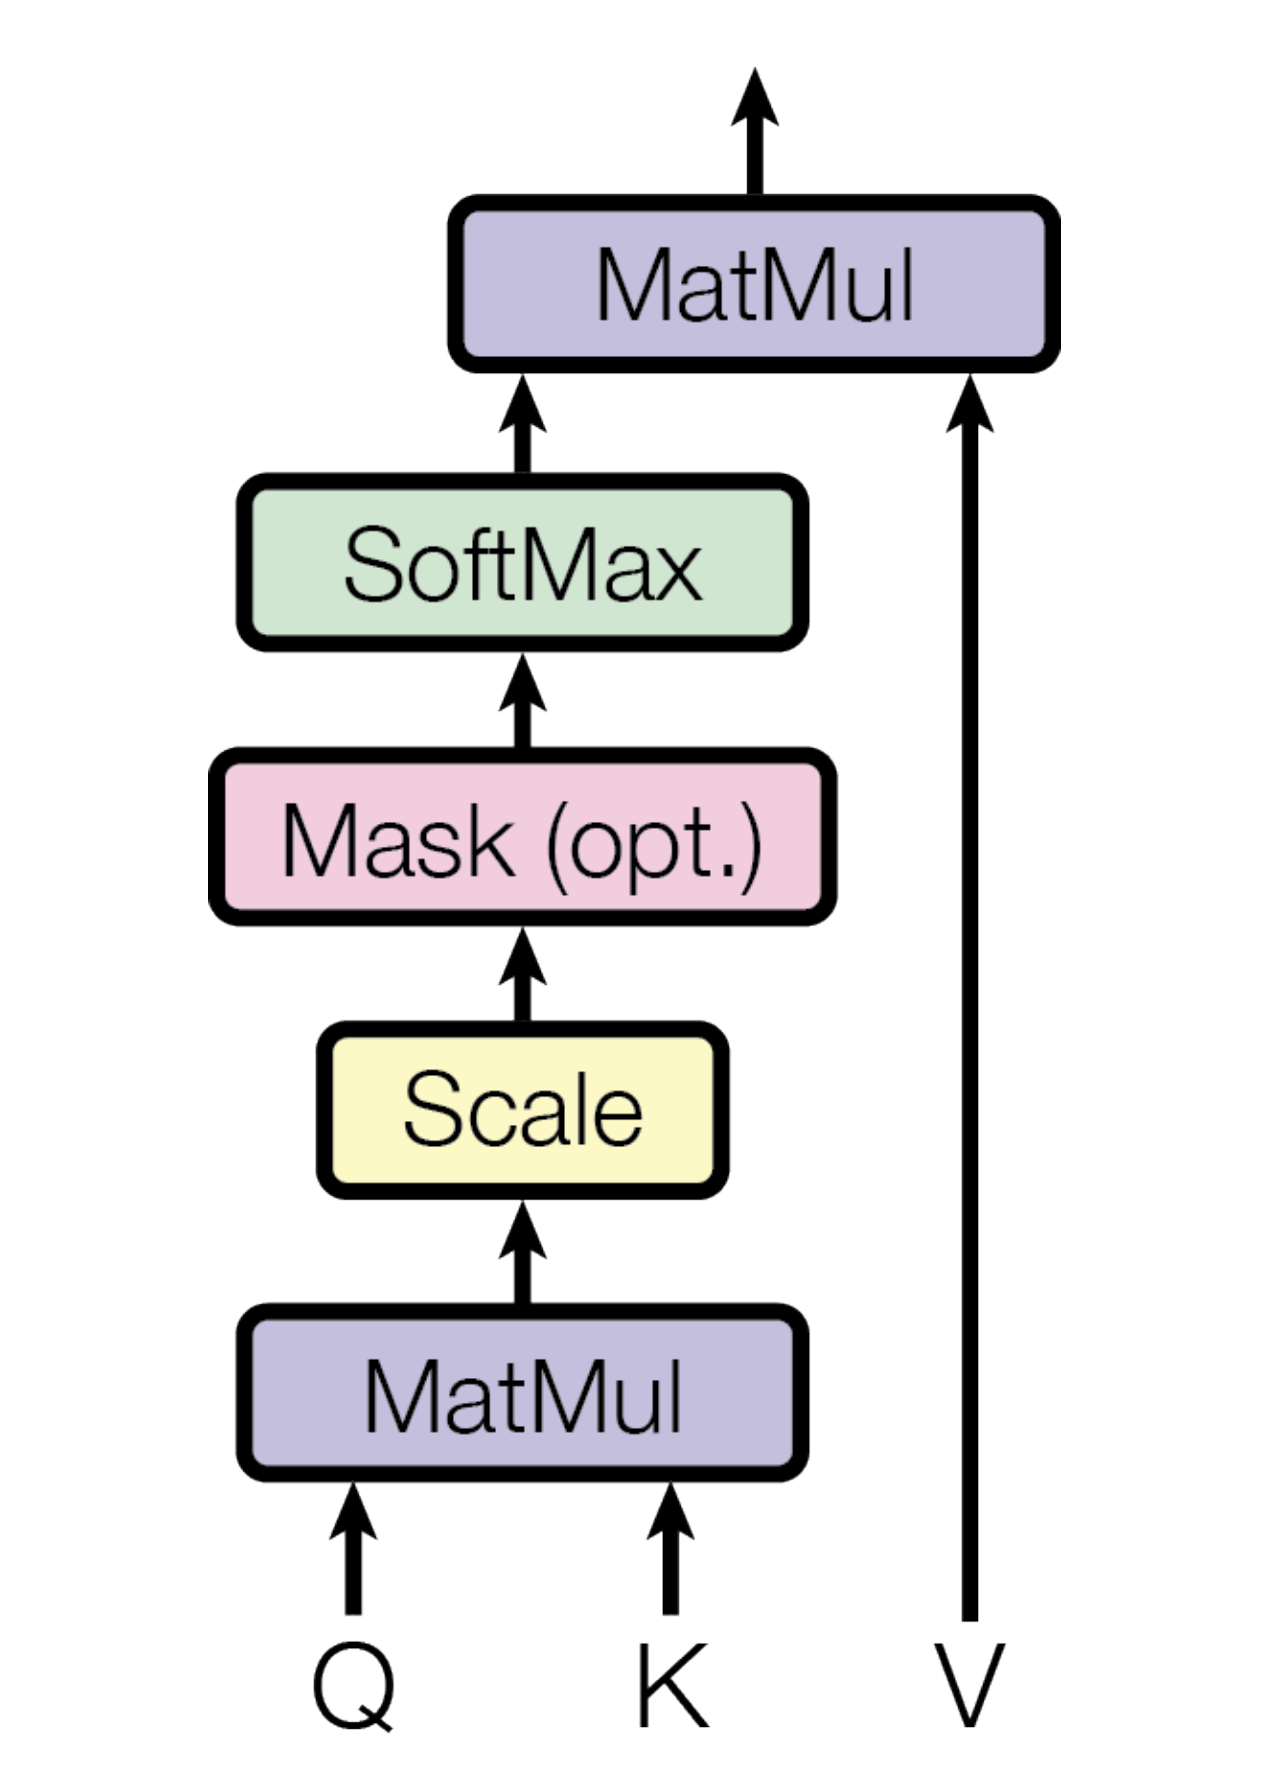
\includegraphics[width=0.5\linewidth]{Image/attn.png}
  \caption{Attention dùng Tich vô hướng}
  \label{fig:self-attn-1}
\end{figure}

Theo như hình \ref{fig:self-attn-2}
Một cách tương tự cho nhiều ma trận thành 1 tensor ta có Multihead Attention được hiểu là:

Thông qua tensor trọng số $W_Q$, $W_K$ ta tính được $Q$,$K$ của x và 

Tương tự với tensor trọng số $W_V$ ta thu được V (value) của y và khi đó. 

Để chuẩn hoá ta sử dụng tham số độ dài của chuỗi nhập vào là $d_k$. Khi đó ta tính dc Attention score (A) như sau:
\begin{center}
$\text {a}= \text {softmax}(\frac{QK^{T}}{\sqrt{d_k}}V)$
\end{center}

\begin{figure}[hbt!]
  \centering
  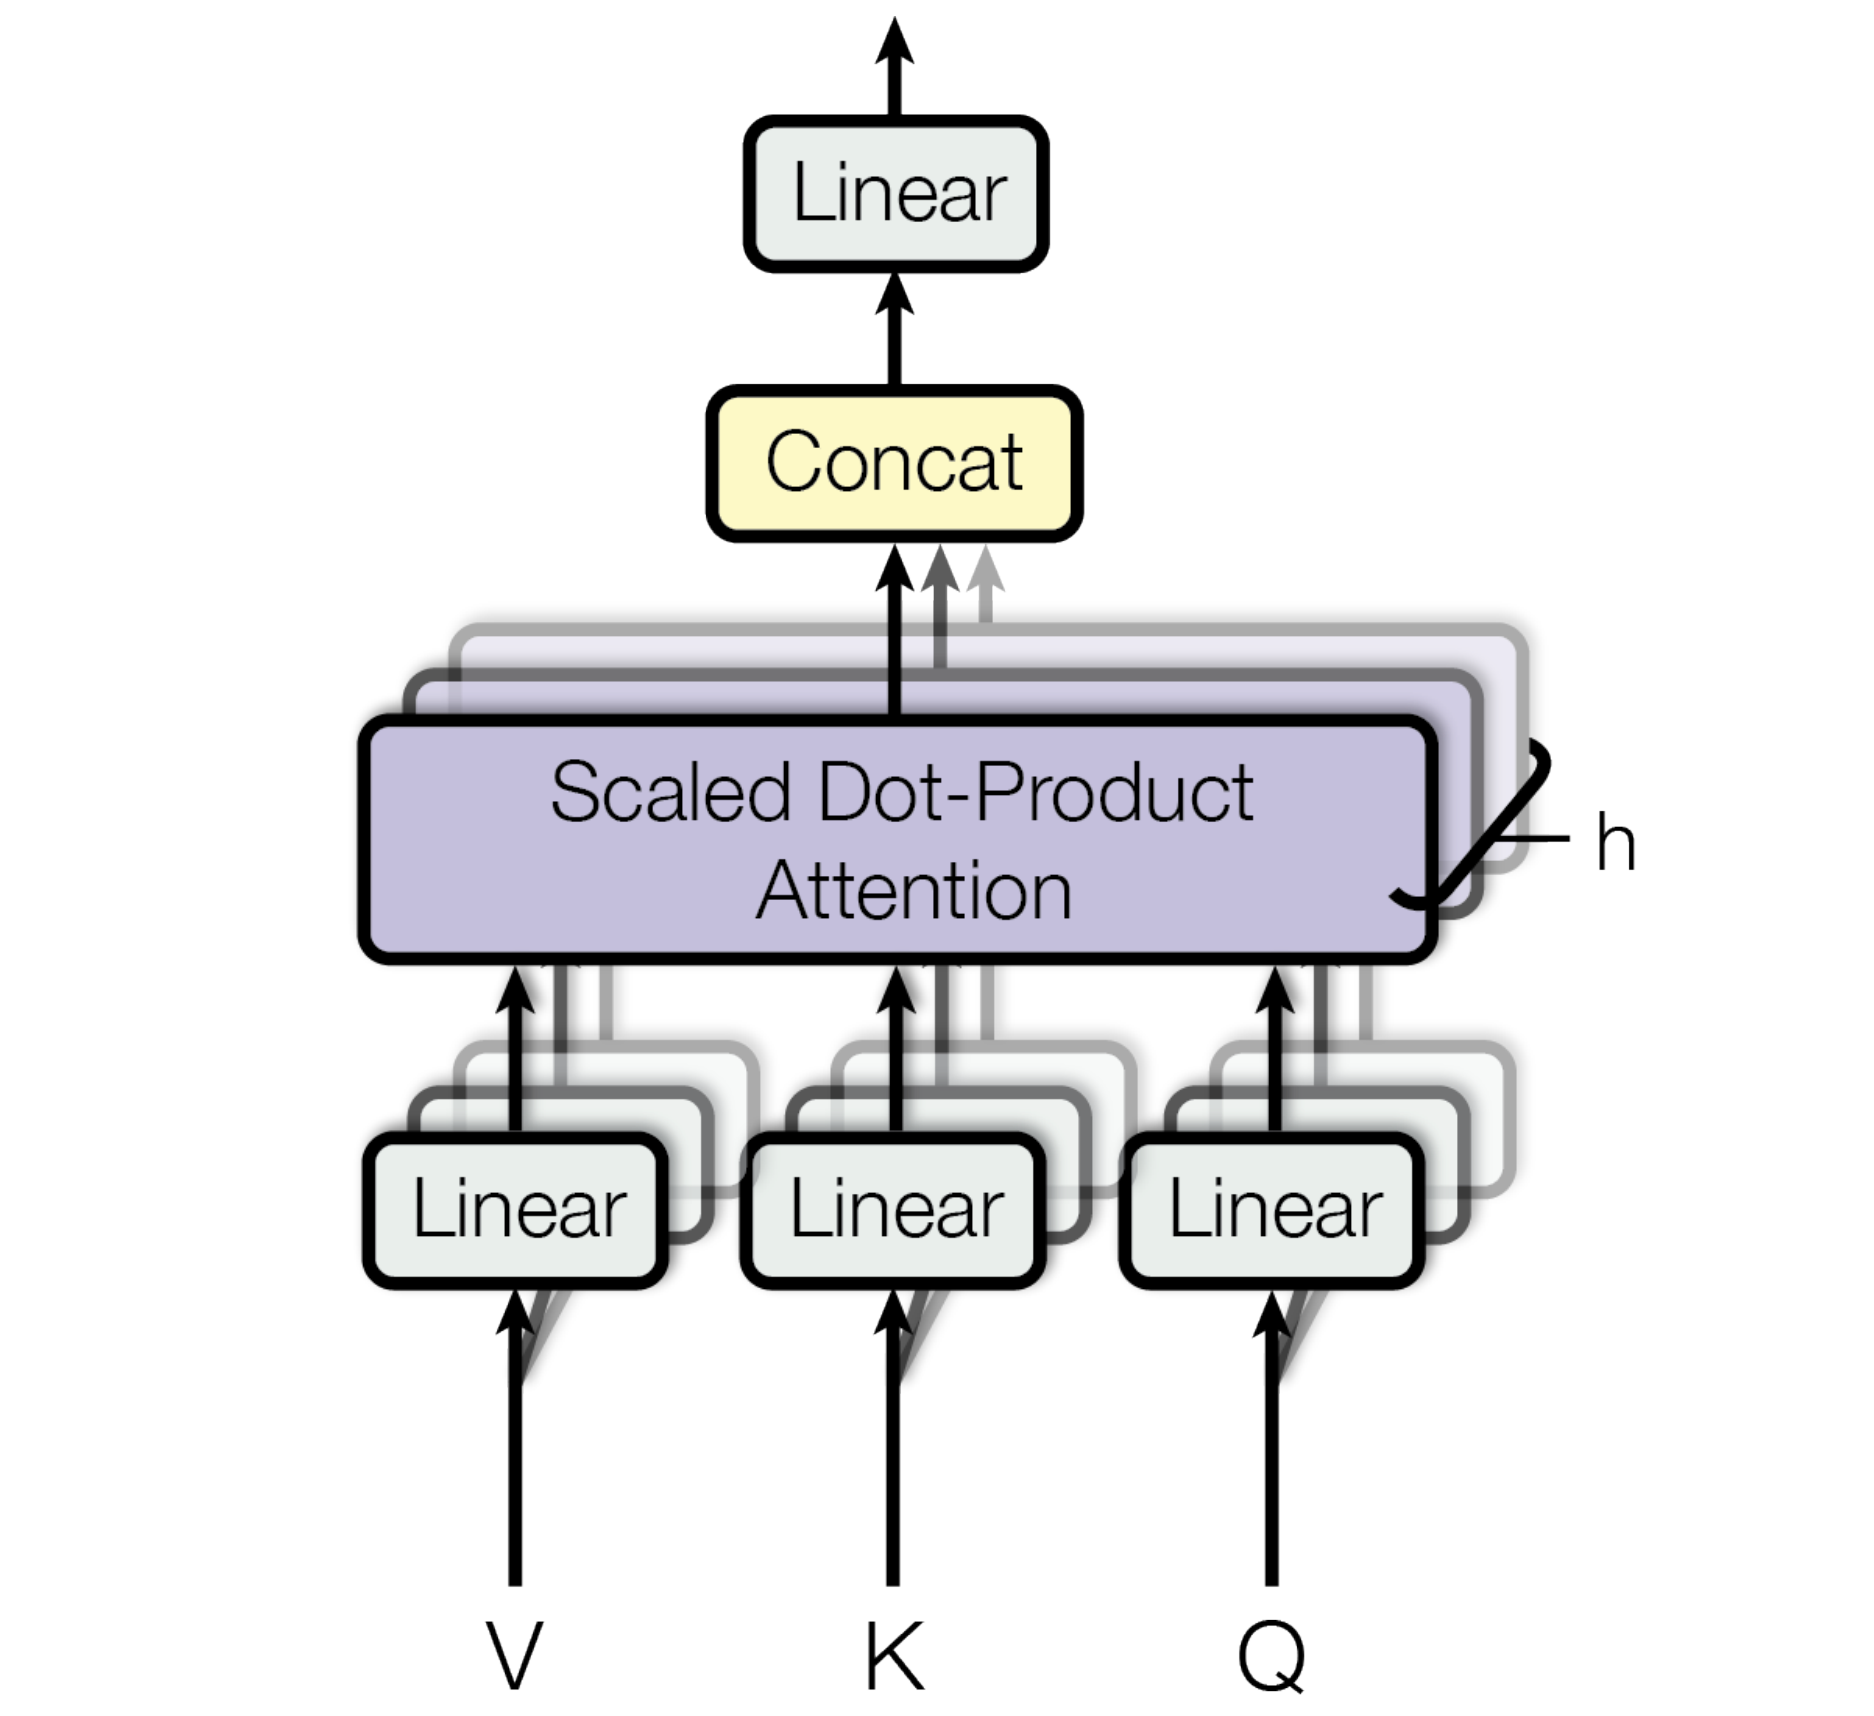
\includegraphics[width=0.5\linewidth]{Image/multi_head_attn.png}
  \caption{Multi-Head Attention}
  \label{fig:self-attn-2}
\end{figure}

Mô hình transformers có bản chất là tìm ra tất cả các mối liên hệ token và 
chính các ma trận trong số lưu giữ các mối liên hệ này như những dạng biểu diễn đặc trưng cho những tính chất nào đó mà câu đó đang mang theo 
dựa vào ngữ liệu và mục tiêu huấn luyện.

Do đó về bản chất mô hình BERT\cite{Devlin2018} như hình \ref{fig:self-attn-3} 
hay RoBERTa\cite{Liu2019} thì là việc chồng chất các quan hệ ẩn dưới dạng các quan hệ được tính bằng attention score và tính chấp nối qua dạng resudial connection như là:
$\text {LayerNorm}(x+\text {Sublayer}(x))$.
\begin{figure}[hbt!]
  \centering
  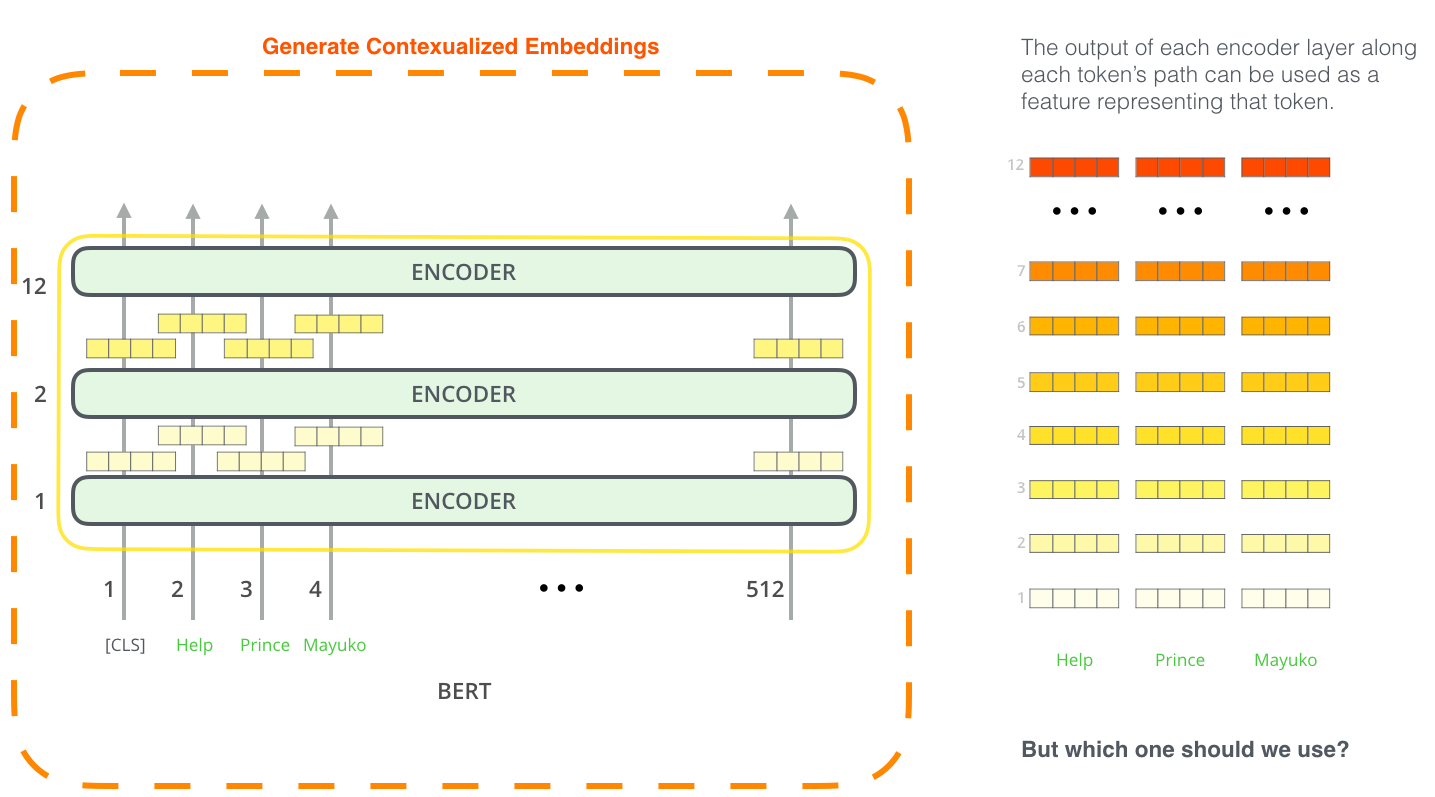
\includegraphics[width=\linewidth]{Image/bert.png}
  \caption{Mô hình Transformers}
  \label{fig:self-attn-3}
\end{figure}

Nhờ vào tính chồng chất và tính tổ hợp của các chồng chất quan hệ biểu diễn trong không gian ẩn mà khi huấn luyện cho các tác vụ đặc định mà mô hình ngôn ngữ yểm mã nói riêng hay 
mô hình ngôn ngữ nói chung tỏ ra vượt trội hơn các tiếp cận cũ \cite{Nguyen2020}.
\subsection{RoBERTa}
RoBERTa\cite{Liu2019} là viết tắt của \textbf{R}obustly \textbf{O}ptimized \textbf{BERT} pretraining \textbf{A}pproach 
là một cách tiếp cận mà chúng tôi sử dụng là khung xương cho toàn bộ mô hình chúng tôi.

\subsection{FasterTransformer}
Để huấn luyện và sử dụng cho các tác vụ đặc định hiệu quả trên những tài nguyên tính toán dùng cho học sâu như GPU.
Chúng tôi nhân thấy việc sử dụng lớp self-attention cho GPU do NVIDIA hỗ trợ phù hợp cho việc tính toán các khối ma trận tối ưu như ở hình \ref{fig:self-attn-5}.
\begin{figure*}[]
  \centering
  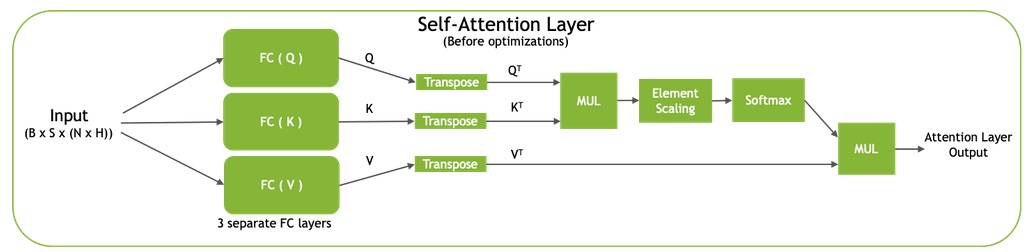
\includegraphics[width=\linewidth]{Image/self_attn_layer_before.jpg}
  \caption[caption]{Lớp Self-Attention thông thường
  \footnote{\url{https://developer.nvidia.com/blog/nlu-with-tensorrt-bert/}}}
  \label{fig:self-attn-4}
\end{figure*}

\begin{figure*}[hbt!]
  \centering
  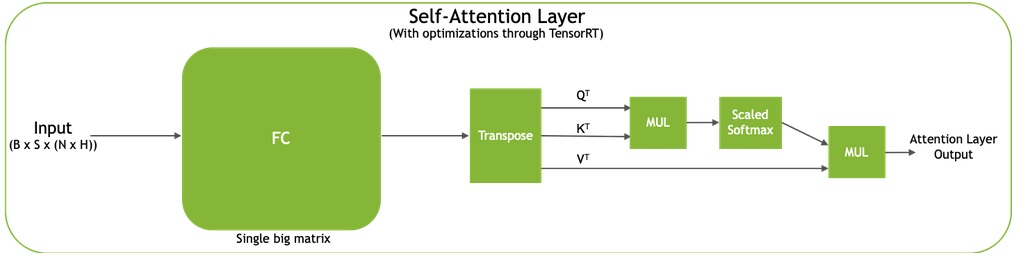
\includegraphics[width=\linewidth]{Image/self_attn_layer.jpg}
  \caption[caption]{Lớp Self-Attention cho GPU sử dụng trong modoule FasterTransformer
  \footnote{\url{https://developer.nvidia.com/blog/nlu-with-tensorrt-bert/}}}
  \label{fig:self-attn-5}
\end{figure*}

Ở hình \ref{fig:self-attn-5} chúng ta thấy rõ sự tối ưu nếu như mô hình được tính toán theo khối ma trận hay tensor một cách song song 
trên GPU giúp tiết kiệm được thời gian tính toán đáng kể.
\subsection{ALBERT}
ALBERT\cite{Lan2019} hay là \textbf{A} \textbf{L}ite \textbf{BERT} là mô hình tuy có số lượng tham số nhỏ hơn \cite{Devlin2018} tuy nhiên lại thể hiện kết quả cải thiện đáng kể so với tiền nhiệm.
Trong mô hình ngôn ngữ chúng tôi sử dụng hai kĩ thuật sau làm nền tảng để bước đầu thu gọn kích thước mô hình như không làm mất mà con tăng dần tính hiệu quả của mô hình.
\subsubsection{Phân giải Embedding (Factorized embedding parameterization)}
Nhằm mục đích giảm nhẹ kích thước mô hình chúng tôi phân giản ma trận tham số embedding thành 2 ma trân nhỏ hơn.
Thay cho thực hiện phép chíêu vector one-hot trên không giản ẩn (hidden space) có kích thước là H, chúng tôi sử dụng hướng dẫn trong paper
ALBERT\cite{Lan2019} là chiếu xuốnng không gian embedding có số chiều là E trước rồi mới chiếu xuống không gian ẩn.
Nhờ vậy nếu $H>>E$ thì số tham số embeddinng sẽ giảm từ $O(V \times H)$ xuống $O(V \times E + E \times H)$
\subsubsection{Cộng hưởng tham số giữa các lớp (Cross-layer parameter sharing)}
Nhằm mục đích tăng tốc qua trình huấn luyện chúng tôi cũng sử dụng những kĩ thuật cộng hưởng tham số và lựa chọn cấu hình của kết quả thí nghiệm tốt nhất đề cập trong \cite{Lan2019}.
Nhờ quá trình cộng hưởng tham số quá trình cập nhật trong số sẽ nhanh hơn và mô hình cũng sẽ càng thêm nhẹ nhàng vì không cần quá nhiều thông số để mà lưu trữ thông tin được phiên mã (encoded) trong mô hình.
\section{Dữ liệu và phương pháp nghiên cứu}
\subsection{Kiến trúc}
Chúng tôi xây dựng bốn mô hình thí nghiệm
\begin{enumerate}
  \item \label{itm:first} Sử dụng mô hình RoBERTa\cite{Liu2019} ở cấu hình base 
  với sự thay đổi là chỉ là 8 lớp Transfomer và độ dài chuỗi đầu vào tối đa 128.
	\item \label{itm:second} Sử dụng mô hình \ref{itm:first} nhưng các lớp Transformers được thay bằng FasterTransformer.
	\item \label{itm:third} Sử dụng mô hình \ref{itm:second} nhưng các lớp lớp Embddining thông thường được thay bằng lớp Embedding được phân giải.
	\item \label{itm:forth} Sử dụng mô hình \ref{itm:third} và Công hướng tham số giữa các lớp sau khi tính toán độ attention trong các lớp dựa vào \cite{Lan2019}.
\end{enumerate}
\subsection{Mục tiêu huấn luyện}
Chúng tôi hoàn toàn sử dụng lại hàm lỗi và mục tiêu huấn luyện chỉ cho tác vụ của mô hình ngôn ngữ yểm mã trong bài báo RoBERTa\cite{Liu2019}.
\subsection{Thuật toán tối ưu}
Do mô hình học không huấn luyện trên TPU (Tensor Processing Unit) 
như cách bài báo ALBERT\cite{Lan2019} sử dụng thuật toán LAMB\cite{You2019}, vì thế để có thể huấn luyện tối ưu với batch size lớn (2048-4096) 
chúng tôi đã sử dụng thuật toán tối ưu tối ưu trên GPU là NVLAMB \ref{alg:nvlamb}.

\begin{algorithm}[!ht]
  \SetAlgoLined
  \KwResult{Trọng số mô hình tại bước $t+1$}
   \textbf{Khởi tạo}: Tại bước $t$ với mini-batch $x$ và trọng số mô hình là $w(t)_{l}^{i}$\\
   \textbf{Bước 1}: Tính đạo hàm $g(t)_{l}^{i}$của trọng số mô hình $w(t)_{l}^{i}$ \\
   \textbf{Bước 2}: Chuẩn hoá đạo hàm:\\
   \begin{center}
    $g(t)= \forall_{l=1}^{L} \text {concatentate}(g(t)_{l})$ \\ 
    $g_{norm}(t)=\|g(t)\|_{2}$\\
   \end{center}
    \eIf{$g_{norm}(t)>1$}{$\widehat{g}(t)_{l}^{i}=\frac{g(t)_{l}^{i}}{g_{norm}(t)}$\\}
    {${g}(t)_{l}^{i}$}
   \textbf{Bước 3}: Cập nhật hàm momentum $m(t)$, hàm vận tốc $v(t)$ tương ứng với
   trọng số của lớp $l$ là $w(t)_{l}^{i}$ dựa trên đạo hàm $g(t)$ và các siêu tham số
   $\beta_{1}$ và $\beta_{2}$:\\
   \begin{equation}
    m(t)_{l}^{i}=\beta_{1} m(t-1)_{l}^{i}+\left(1-\beta_{1}\right) \widehat{g}(t)_{l}^{i}
   \end{equation}
   \begin{equation}
    v(t)_{l}^{i}=\beta_{2} m(t-1)_{l}^{i}+\left(1-\beta_{2}\right) (\widehat{g}(t)_{l}^{i})^{2}
   \end{equation}
   \textbf{Bước 4}: Áp dụng beta-correction:
   \begin{equation}
    \widehat{m}(t)_{l}^{i}=\frac{m(t)_{l}^{i}}{\left(1-\left(\beta_{1}\right)^{t}\right)}
   \end{equation}
   \begin{equation}
    \widehat{v}(t)_{l}^{i}=\frac{v(t)_{l}^{i}}{\left(1-\left(\beta_{2}\right)^{t}\right)}
   \end{equation}
   \textbf{Bước 5}: Cập nhật $u(t)_{l}^{i}$ dựa vào trọng số $w(t)_{l}^{i}$ dựa vào tham số $\lambda$ và $\epsilon$:
   \begin{center}
    $u(t)_{l}^{i}=\frac{\widehat{m}(t)_{l}^{i}}{\sqrt{\widehat{v}(t)_{l}^{i}+\epsilon}}+\lambda w(t)_{l}^{i}$
   \end{center}
   \textbf{Bước 6}: Tính tỉ lệ $r(t)_{l}$ giữa trọng số $w(t)_{l}$ và độ lớn của tham số cập nhật $u(t)_{l}$:
   \begin{center}
    $r(t)_{l}=\frac{\left\|w(t)_{l}\right\|_{2}}{\left\|u(t)_{l}\right\|_{2}}$
   \end{center}
   \textbf{Bước 7}: Cập nhật trọng số $w(t)_{l}$ và tốc độ học (learning rate) $lr$:
   \begin{center}
    $w(t+1)_{l}^{i}=w(t)_{l}^{i}- lr \times r(t)_{l} \times u(t)_{l}^{i}$
   \end{center}
   \caption{Thuật toán tối ưu NVLAMB dùng cho GPU}.
   \label{alg:nvlamb}
  \end{algorithm}
\subsection{Dữ liệu}
\label{dataset}
Chúng tôi tiến hành sử dụng ngữ liệu tin tức miễn phí như đã trình bày trong \ref{introduction} và 
tiến hành lọc và tách các từ theo thuật toán\ref{alg:corpus}:
\begin{algorithm}[!ht]
  \SetAlgoLined
  \KwResult{Ngữ liệu và từ điển cho huấn luyện mô hình ngôn ngữ.}
   \textbf{Khởi tạo}: Ngữ liệu huấn luyện theo và kiểm thử đã nêu ở \ref{introduction}.\\
   \textbf{Bước 1}: Lược bỏ các dòng trùng lặp.\\
   \textbf{Bước 2}: Kiểm tra tính hợp lệ của câu tiếng Việt theo thuật toán Trích lọc tiếng Việt
   \footnote{\url{http://viet.jnlp.org/cac-cong-cu-xu-ly/trich-loc-tieng-viet-tu-html}}.\\
   \textbf{Bước 3}: Tách ngữ liệu thành dạng mỗi dòng một câu.\\
   \textbf{Bước 4}: Tạo từ điển và tách câu thành dạng token-id vector bằng thuật toán byte-pair-encoding (BPE)\cite{Sennrich2015}.\\
   \textbf{Bước 5}: Lựa chọn các câu mà số phần tử token-id vector nhỏ hơn 128.\\
   \caption{Thuật toán khai thác và tách từ để tạo ngữ liệu cho huấn luyện mô hình ngôn ngữ.}
   \label{alg:corpus}
  \end{algorithm}

Trong quá trình thực nghiệm nhiều lần, chúng tôi nhận ra việc tiền xử lý có vai trò dần quan trọng và không thể bỏ đi dù cho mô hình học sâu có tiên tiến đến đâu.
Chúng tôi đang nghiên cứu và cải thiện dần thuật toán tạo bộ ngữ liệu chuẩn phù hợp nhất các yếu tố ngôn ngữ hoc của tiếng Việt.



\subsection{Quá huấn luyện}

\section{Thí nghiệm và Kết quả}
Chúng tôi thực nghiệm huấn luyện mô hình trên cấu hình máy tính với 
16 CPU Intel(R) Xeon(R) Gold 6130 CPU @ 2.10GHz và 4 GPU NVIDIA Tesla V100 - 32GB VRAM. 
Framework dùng để huấn luyện là Pytorch sử dụng một phần mã nguồn của HuggingFace-Transformers\cite{Taylor1953} 
và NVIDIA-DeepLearningExamples\footnote{\url{https://github.com/NVIDIA/DeepLearningExamples/}}.
Thời gian huấn luyện mô hình trung bình là 12 ngày. 
Chúng tôi sử dụng ngữ liệu huấn luyện và kiểm thử theo những dữ liệu công khai đã được trình bày trong \ref{dataset}.
Kết quả thực nghiệm nhiều mô hình ngôn ngữ có hỗ trợ tiếng việt được trình bày ở Bảng \ref{Bảng:1}
\begin{table*}
  \centering
  \begin{tabular}{|l|l|l|l|}
  \hline
  \textbf{ID} & \textbf{Language Model}                                                       & \textbf{Parameters} & \textbf{Perplexity} \\ \hline
  1           & xlm-roberta-base                                                              & 278.89M             & 495.39              \\ \hline
  2           & xlm-roberta-large                                                             & 561.19M             & 13.16               \\ \hline
  3           & bert-base-multilingual-uncased                                                & 168.05M             & 167.2               \\ \hline
  4           & bert-base-multilingual-cased                                                  & 178.57M             & 78.77               \\ \hline
  5           & distilbert-base-multilingual-cased                                            & 135.45M             & 454.15              \\ \hline
  6           & pho-bert-base                                                                 & 135.65M             & 81.74               \\ \hline
  7           & pho-bert-large                                                                & 370.27M             & 65.19               \\ \hline
  8           & vietnamese-roberta-cased                                                      & 37.68M              & 99.24               \\ \hline
  9           & vietnamese-roberta-uncased                                                    & 34.58M              & 138.44              \\ \hline
  10          & albert-vi                                                                     & 18.11M              & 560.08              \\ \hline
  11          & roberta-base (ours)                                                           & 111.04M             & 31.24               \\ \hline
  12          & roberta-base (FasterTransformer) (ours)                                       & 92.59M              & 24.97               \\ \hline
  13          & roberta-base (FasterTransformer) + cross-layer (ours)                         & 80.82M              & 16.30               \\ \hline
  14          & roberta-base (FasterTransformer) + cross-layer  + factorized embedding (ours) & 76.79M              & \textbf{12.11}      \\ \hline
  \end{tabular}
  \caption{Kết quả thực nghiệm trên tập kiểm thử}
  \label{Bảng:1}
  \end{table*}


\section{Kết luận}

\section*{Cảm tạ}

\bibliographystyle{IEEEtran}
\bibliography{bare_ref}

% that's all folks
\end{document}


